In this section we focus on \cref{fig:LZYandbsweepwide}, \ref{fig:LZYandbsweepnarrow}, and \ref{fig:LZYandbsweepfractal} which we used to find the quasi-periodic orbits we showed in a previous section. To create \cref{fig:LZYandbsweepwide} we computed trajectories for varying initial conditions and parameter $b$, specifically, we computed the trajectories for:
\begin{align*}
\left(\frac{1}{2}+\sqrt{R^2-\left(y-\frac{1}{2}\right)^2} , y, 1, 0\right) 
&\text{ for } y\in \frac{1}{2}+ 0.32\cdot [-1,1],\\ 
&\text{ and } b\in [0.001, 5],
\end{align*}
where we sampled $y$ and $b$ in 500 equidistant points, and the trajectories were computed to a depth of 128 iterations. For \cref{fig:LZYandbsweepnarrow} we did the same except we varied $b\in[0.1,1]$. The color in the plots indicates the LZC of the sampled trajectory. From the colorbar on the right, we see blue indicates low LZC, red intermediate, and yellow high LZC. The colors are scaled between the lowest and highest LZC in the plot, so colors in separate plots may vary. Also, notice the colorbar is scaled logarithmically, this improves legibility.

We immediately notice large regions of uniformly low LZC scattered across the plots, these suggest regions of stable quasi-periodic behavior. This is corroborated by the fact that in \cref{fig:LZYandbsweepwide} the trajectory for $(y,b)=(1/2,3)$, corresponding to the periodic orbit in \cref{subfig:penandpaperorbits1}, lands inside one of these low LZC regions, and far from the boundary. In fact, the initial conditions for all of the quasi-periodic orbits we discovered can be found in either of these plots. 
\begin{figure}[!th]
\centering
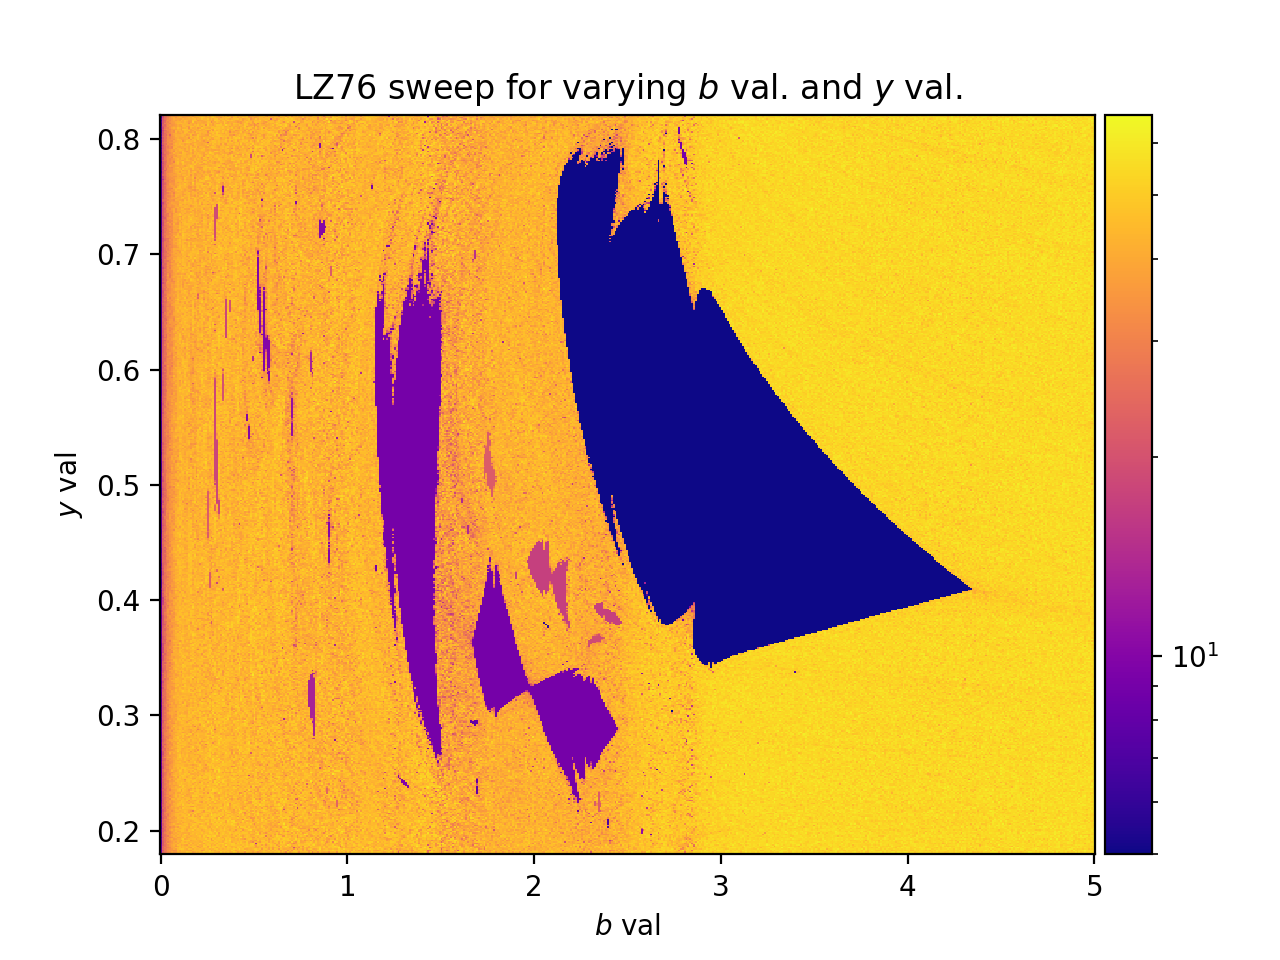
\includegraphics[width=0.9\textwidth, trim={0.5cm 0cm 0cm 0.5cm}, clip]{LZ_b_Y_sweep.png}
\caption{LZC for a 2-d slice of initial conditions}
\label{fig:LZYandbsweepwide}
\end{figure}

We note the color of the regions differs, indicating that the behavior producing the regions is qualitatively different. The regions do not seem to be arranged in any specific pattern, yet they all seem to have a similar structure: that being 1, 2, or 3 ``bulbs''. It might be that the number of bulbs may change depending on the resolution of the plot and depth of the interations. \Cref{fig:LZYandbsweepnarrow} also suggests quasi-periodic trajectories exist for a large range of $b$, also for $b$ in the range of our KAM results.
\begin{figure}[!th]
\centering
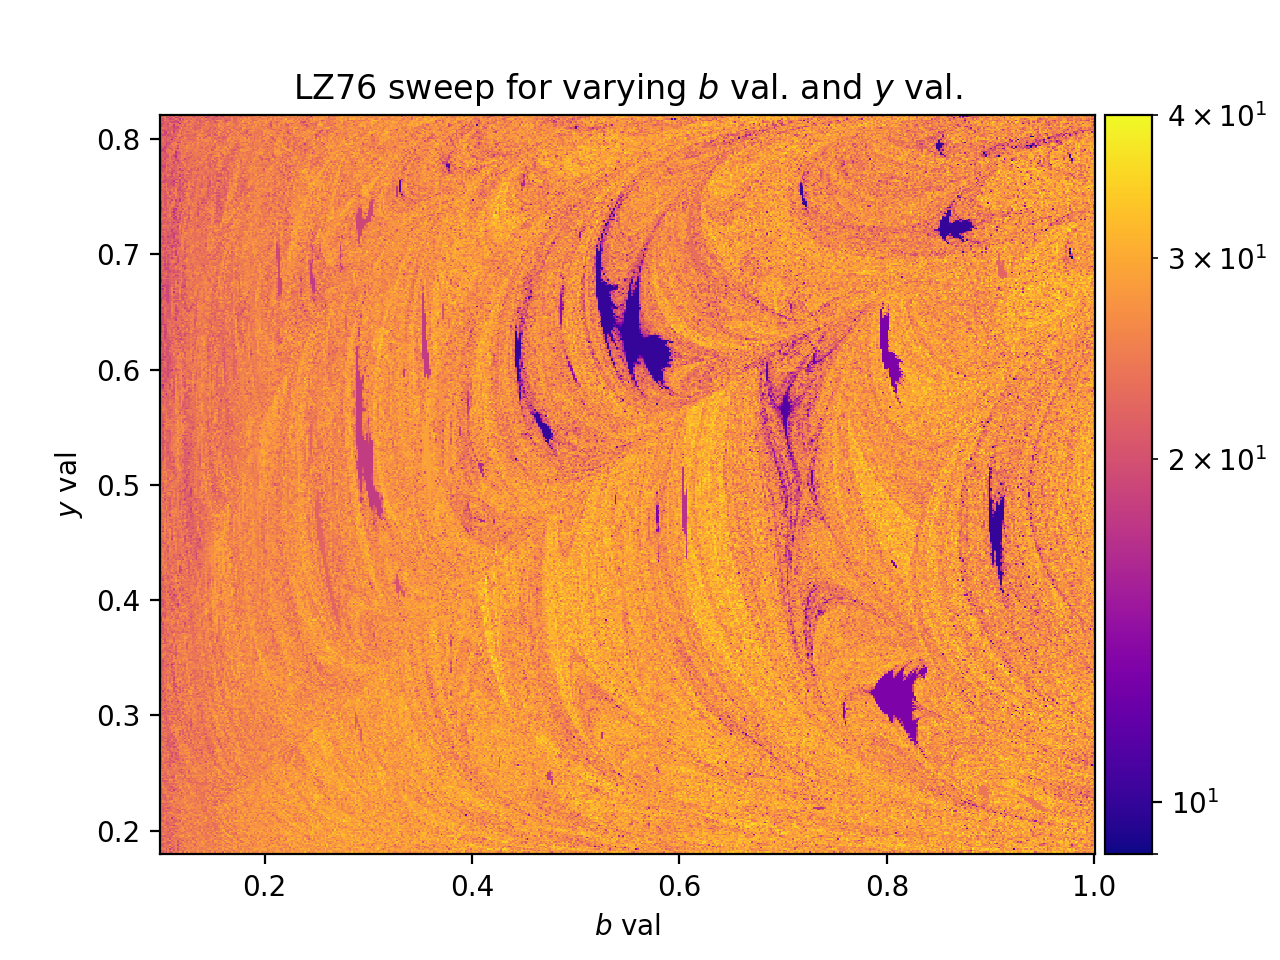
\includegraphics[width=0.9\textwidth, trim={0.5cm 0cm 0cm 0.5cm}, clip]{LZ_b_(01_1)_Y_sweep.png}
\caption{LZC for a narrower 2-d slice of initial conditions}
\label{fig:LZYandbsweepnarrow}
\end{figure}

If we repeat the same analysis for smaller $b$, the details are harder to discern. Focusing on $b\in(0.2,0.4)$ in \cref{fig:LZYandbsweepnarrow}, we still see the stable regions as before, however the color blends with the surrounding noise. This can be explained by the effect mentioned: the period of the trajectories is comparable to the time horizon, so periodicity is less distinguishable from noise.

Lastly, we discuss the boundary of the regions. Note that for $b\in(2,3)$ and $y\in(0.7, 0.8)$ the plot seems grainy, in fact, zooming in, we find fractal-like behavior which can be seen in \cref{fig:LZYandbsweepfractal}. This is in contrast to the rest of the boundary which seems differentiable. We do not provide a figure but zooming in on the boundary for $b\in (3,4)$ we see it is also grainy. It is not clear whether the noise is due to intrinsic structure or precision error.

\begin{figure}[!th]
\centering
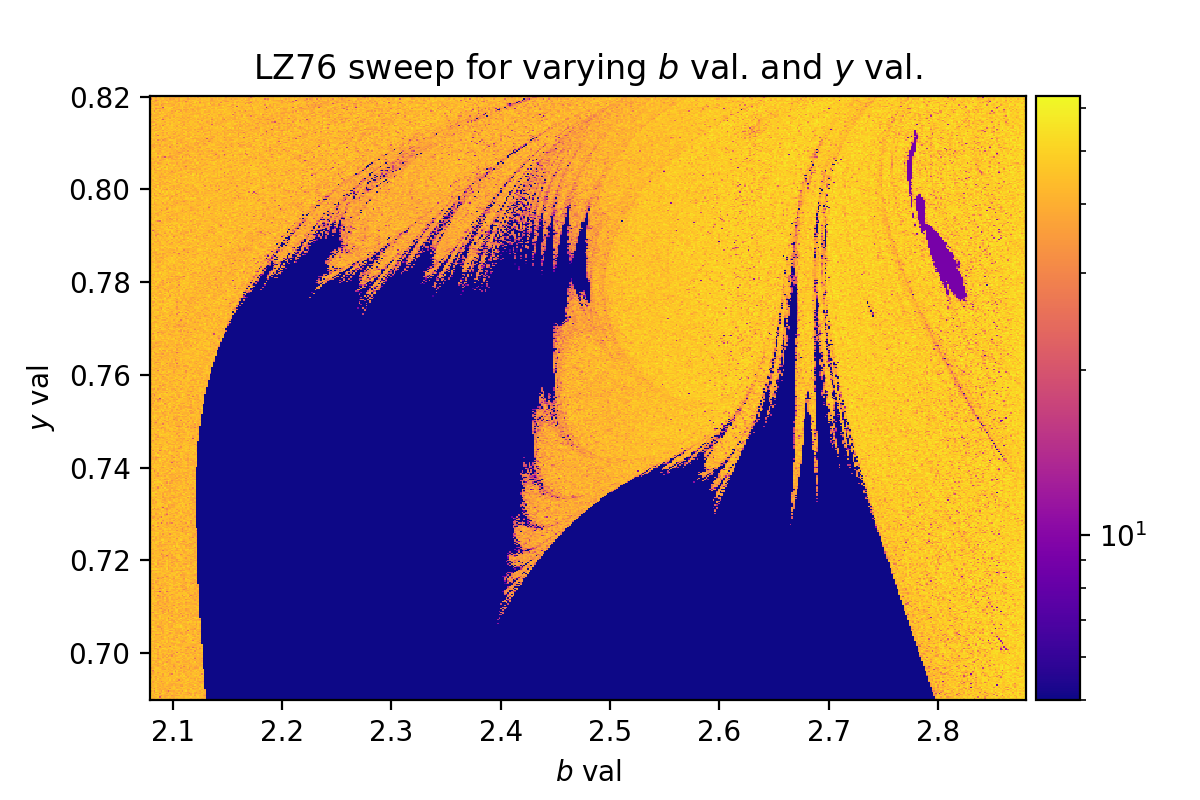
\includegraphics[width=\textwidth, trim={0cm 0cm 0cm 0cm}, clip]{LZ_b_Y_sweep_fractals.png}
\caption{Fractal-like structure arising from Lempel-Ziv complexity}
\label{fig:LZYandbsweepfractal}
\end{figure}

Apart from regions of stability, there is a sea of high and noisy LZC throughout the plots. Closer inspection shows specks with low LZC, it is not clear whether these specks are trajectories like \cref{fig:sensitive_trajectory} or if they correspond to quasi-periodic regions with a very small radius of stability. Focusing on \cref{fig:LZYandbsweepwide}, there is a peculiar vertical line at $b\approx2.8$. On the right of this line the average LZC looks higher than to the left, we are curious whether there is any significance to this or if it is just a coincidence. Lastly, we also checked the plot for $b\in(5,10)$ and found the same behavior as $b\in(4.3, 5)$: high LZC with no stable regions.

Using symbolic dynamics together with LZC we have probed a rich landscape of behavior. The choice of initial conditions and parameters for the above figures was deliberate, so it is interesting to ask whether we can expect a similar landscape for other choices. For example, will the view change if we vary velocity at a point, or if we pick a different radius $R\neq1/3$. There are many option, and we invite the reader to explore as well.